% (C) Copyright 2016
% Urs Fässler, www.bitzgi.ch
% SPDX-License-Identifier: CC-BY-SA-4.0

\subsection{Lizenzen}
\label{sec:lizenzen}
\subsectionframe

\begin{frame}{Lizenz-Kategorien}
	\begin{center}
		\begin{tabular}{ccc}
		
\includegraphics[width=2.5cm]{res/PD-icon.pdf} & 
\includegraphics[width=2.5cm]{res/by.pdf} & 
\includegraphics[width=2.5cm]{res/copyleft.pdf} \\ 
		Public Domain & Permissiv & Copyleft \\
		\hspace{3cm} & \hspace{3cm} & \hspace{3cm} \\
		\end{tabular} 
	\end{center}
\end{frame}
\note
{
	\begin{itemize}
		\item Copyleft, viral: https://de.wikipedia.org/wiki/Copyleft
	\end{itemize}
}

\begin{frame}{Kategorien Gegenüberstellung}
	\newcommand{\yes}{\color{green}\checkmark}
	\newcommand{\no}{\boldmath \color{red}$\times$}
	\begin{tabular}{lccc}
		& 
\includegraphics[width=1cm]{res/PD-icon.pdf} & 
\includegraphics[width=1cm]{res/by.pdf} & 
\includegraphics[width=1cm]{res/copyleft.pdf} \\ 
		& Public Domain & Permissiv & Copyleft \\ 
		\hline 
		Freie Software & \yes & \yes & \yes \\ 
		\hline 
		Kommerziell & \yes & \yes & \yes \\ 
		\hline 
		Proprietär & \yes & \yes & \no \\ 
		\hline 
		Code veröffentlichen & \no & \no & \yes \\ 
		\hline 
		Copyright angeben & \no & \yes & \yes \\ 
		\hline 
		Lizenz mitliefern & \no & \yes & \yes \\ 
		\hline 
		gültig in D-A-CH & \no & \yes & \yes \\
		\hline 
	\end{tabular} 
\end{frame}{

\begin{frame}{Public Domain Lizenzen}
	
\includegraphics[height=3cm]{res/PD-icon.pdf}
	\hfill
	
\includegraphics[height=3cm]{res/beer.pdf}
	\hfill
	
\includegraphics[height=2.5cm]{res/WTFPL_logo.pdf}
	\\
	
\includegraphics[width=4cm]{res/cc-zero.pdf}
\end{frame}
\note
{
	\begin{itemize}
		\item The Unlicense (\url{http://programmers.stackexchange.com/questions/147111/what-is-wrong-with-the-unlicense\#147120})
		\item Beerware
		\item Beer: CC-0 by drunken\_duck (\url{https://openclipart.org/detail/2214/beer})
		\item WTFPL (\url{https://en.wikipedia.org/wiki/WTFPL})
		\item An official logo for the WTFPL license: WTFPD by www.wtfpl.net \url{https://commons.wikimedia.org/wiki/File:WTFPL_logo.svg}
		\item nicht gültig in D-A-CH
		\item Verwende CC-0
		\item CC-0: Public Domain (\url{https://creativecommons.org/about/downloads/})
	\end{itemize}
}

\begin{frame}{Permissive Lizenzen}
	\begin{center}
		{\Huge MIT}
		\hfill
		{\Huge BSD}
		\hfill
		{\Huge Apache}
		\\
		
\includegraphics[width=4cm]{res/cc-by.pdf}
	\end{center}
\end{frame}
\note
{
	\begin{itemize}
		\item MIT, BSD, Apache
		\item Darf
		\begin{itemize}
			\item Ist generell Freie Software
			\item Kommerzielle Verwendung
			\item Proprietäre Verwendung
		\end{itemize}
		\item Muss
		\begin{itemize}
			\item Copyright angeben
			\item Lizenz mitliefern
		\end{itemize}
		\item CC-BY: Public Domain (\url{https://creativecommons.org/about/downloads/})
	\end{itemize}
}

\begin{frame}{Copyleft Lizenzen}
	\begin{center}
		
\includegraphics[height=1.5cm]{res/gpl-v3-logo.pdf}
		\hfill
		
\includegraphics[height=1.5cm]{res/lgpl-v3-logo.pdf}
		\hfill
		
\includegraphics[height=1.5cm]{res/agpl-v3-logo.pdf}
		\\
		
\includegraphics[width=4cm]{res/cc-by-sa.pdf}
	\end{center}
\end{frame}
\note
{
	\begin{itemize}
		\item GPL, LGPL, AGPL, MPL
		\item Darf
		\begin{itemize}
			\item Ist generell Freie Software
			\item Kommerzielle Verwendung
		\end{itemize}
		\item Darf nicht
		\begin{itemize}
			\item Proprietäre Verwendung
		\end{itemize}
		\item Muss
		\begin{itemize}
			\item Code veröffentlichen
			\item Copyright angeben
			\item Lizenz mitliefern
		\end{itemize}
	\end{itemize}
	\begin{itemize}
		\item GPLv3 Logo: Public Domain by Free Software Foundation (\url{https://commons.wikimedia.org/wiki/File:GPLv3\_Logo.svg})
		\item LGPLv3 Logo: Public Domain by Free Software Foundation (\url{https://commons.wikimedia.org/wiki/File:LGPLv3\_Logo.svg})
		\item AGPLv3 Logo: Public Domain by Free Software Foundation (\url{https://commons.wikimedia.org/wiki/File:AGPLv3\_Logo.svg})
		\item CC-BY-SA: Public Domain (\url{https://creativecommons.org/about/downloads/})
	\end{itemize}
}

\begin{frame}{Detailliertere Informationen}
	\begin{itemize}
		\item \url{https://tldrlegal.com/}
	\end{itemize}
	\vspace{1em}
	\begin{center}
		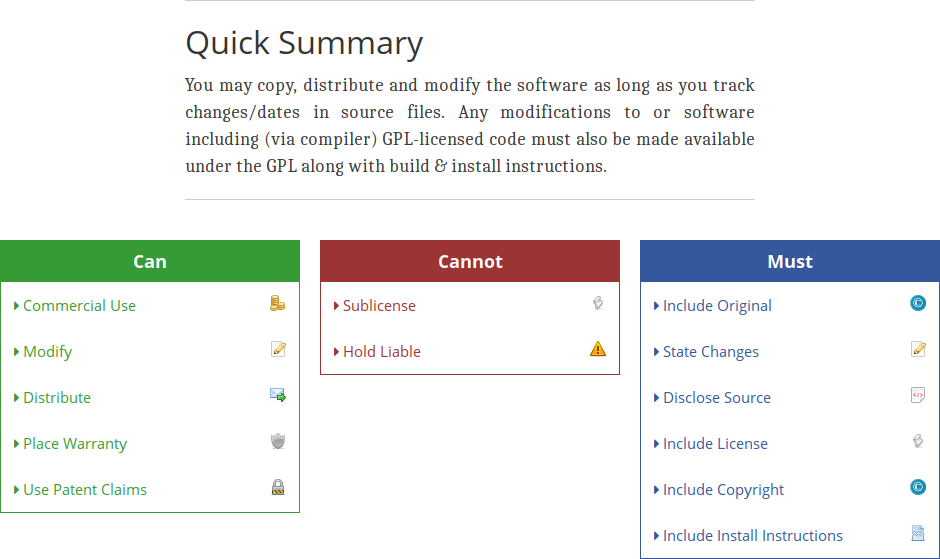
\includegraphics[height=5cm]{res/tldrlegal.png}
	\end{center}
\end{frame}
